\documentclass[journal=jctcce,manuscript=article]{achemso}
%\documentclass[preprint]{revtex4-1}
%\documentclass[11pt]{article}
\usepackage[version=3]{mhchem} % Formula subscripts using \ce{}
\usepackage[T1]{fontenc}       % Use modern font encodings

\renewcommand*{\thefootnote}{\alph{footnote}}

\usepackage{amsmath,amsfonts,graphicx,subfigure}
\usepackage{enumitem}
\usepackage{calc}       
\usepackage{xfrac}     
\usepackage{relsize}

%\bibliographystyle{unsrt}
%\bibliographystyle{achemso}
%-------------- formating ----------------------
\newlength{\figwidth}
\setlength{\figwidth}{0.45\textwidth}
\newcommand{\figpath}{Figures}
\setlength{\itemsep}{0pt}
%-------------- editing ----------------------
\usepackage[usenames,dvipsnames]{xcolor}
\newcommand{\comment}[1]{\textcolor{blue}{[ \sc{#1} ]}} % comments
\newcommand{\revise}[1]{\textcolor{red}{{#1}}} % revisions
\renewcommand{\labelitemi}{$\circ$}
\newcommand{\done}{$\bullet$}
%-------------- draft ----------------------
%\setlength{\fboxrule}{1pt}%
%\newcommand{\todo}[1]{\fbox{\parbox{0.8\textwidth}{ {\bf to do:}{{#1}}}}}
%\usepackage{fancyhdr}
%\pagestyle{fancyplain}
%\lhead{}
%\chead{\textcolor{red}{RE Jones \ \today \ {\bf DRAFT} \ \sc{Please do not redistribute}}}
%\rhead{}
%-------------- aliases -----------------------
\newcommand{\aref}[1]{{App. \ref{#1}}}
\newcommand{\eref}[1]{{Eq. (\ref{#1})}}
%% in natbib \citet will display the authors
\newcommand{\cref}[1]{{Ref. \citenum{#1}}}
%\newcommand{\cref}[1]{{Ref. \cite{#1}}}
\newcommand{\sref}[1]{{Sec. \ref{#1}}}
\newcommand{\fref}[1]{{Fig. \ref{#1}}}
%\newcommand{\cf}{{\it cf.\ }}
\newcommand{\ie}{{\it i.e.\ }}
\newcommand{\vs}{{\it vs.\ }}
\newcommand{\eg}{{\it e.g.\ }}
\newcommand{\etc}{{\it etc.\ }}
\newcommand{\etal}{{\it et al.\ }}
\newcommand{\apriori}{{\it a priori }}
\newcommand{\abinitio}{{\it ab initio }}
\newcommand{\viceversa}{{\it vice versa}}
%...............................................
\newcommand{\smallDelta}{\mathsmaller{\mathsmaller{\Delta}}}
\newcommand{\dx}{{\mathsmaller{\mathsmaller{\Delta}}}\mathbf{x}}
\newcommand{\dt}{{\mathsmaller{\mathsmaller{\Delta}}}{t}}
\newcommand{\neighborhood}{\mathcal{C}}
\newcommand{\grad}{{\boldsymbol{\nabla}}}
\newcommand{\sigmab}{{\boldsymbol{\sigma}}}
\newcommand{\Upsilonb}{{\boldsymbol{\Upsilon}}}
\newcommand{\Phib}{{\boldsymbol{\Phi}}}
\newcommand{\epsilonb}{{\boldsymbol{\epsilon}}}
\newcommand{\spn}{\operatorname{span}}
\newcommand{\tr}{\operatorname{tr}}
\newcommand{\RMSD}{\operatorname{RMS-D}}
\newcommand{\SVD}{\operatorname{SVD}}
\newcommand{\Ball}{\mathcal{B}}
\newcommand{\argmin}{\operatorname{argmin}}
\newcommand{\argmax}{\operatorname{argmax}}
\newcommand{\card}{\operatorname{card}}
\newcommand{\dVx}{\mathrm{d}^3x}
%~~~~~~~~~~~~~~~~~~~~~~~~~~~~~~~~~~~~~~~~~~~~~~~
\newcommand{\dV}{\mathrm{d}V}
\renewcommand{\Im}{\operatorname{Im}}
\newcommand{\Ab}{\mathbf{A}}
\newcommand{\Ac}{\mathcal{A}}
\newcommand{\As}{\mathsf{A}}
\newcommand{\Bc}{\mathcal{B}}
\newcommand{\Cc}{\mathcal{C}}
\newcommand{\Gc}{\mathcal{G}}
\newcommand{\ab}{\mathbf{a}}
\newcommand{\bb}{\mathbf{b}}
\newcommand{\cb}{\mathbf{c}}
\newcommand{\db}{\mathbf{d}}
\newcommand{\eb}{\mathbf{e}}
\newcommand{\fb}{\mathbf{f}}
\newcommand{\kb}{\mathbf{k}}
\newcommand{\vb}{\mathbf{v}}
\newcommand{\Ep}{\mathbb{E}}
\newcommand{\yb}{\mathbf{y}}
\newcommand{\xb}{\mathbf{x}}
\newcommand{\ub}{\mathbf{u}}
\newcommand{\rb}{\mathbf{r}}
\newcommand{\pb}{\mathbf{p}}
\newcommand{\Xb}{\mathbf{X}}
\newcommand{\Xs}{\mathsf{X}}
\newcommand{\ws}{\mathsf{w}}
\newcommand{\Wb}{\mathbf{W}}
\newcommand{\rs}{\mathsf{r}}
\newcommand{\Rs}{\mathsf{R}}
\newcommand{\Rb}{\mathbf{R}}
\newcommand{\Ib}{\mathbf{I}}
\newcommand{\Js}{\mathsf{J}}
\newcommand{\Is}{\mathsf{I}}
\newcommand{\Kb}{\mathbf{K}}
\newcommand{\Pb}{\mathbf{P}}
\newcommand{\Ps}{\mathsf{P}}
\newcommand{\Ub}{\mathbf{U}}
\newcommand{\Us}{\mathsf{U}}
\newcommand{\Vb}{\mathbf{V}}
\newcommand{\Vs}{\mathsf{V}}
\newcommand{\Yb}{\mathbf{Y}}
\newcommand{\Ys}{\mathsf{Y}}
\newcommand{\Ws}{\mathsf{W}}
\newcommand{\Ss}{\mathsf{S}}
\newcommand{\Sb}{\mathbf{S}}
\newcommand{\Db}{\mathbf{D}}
\newcommand{\Ds}{\mathsf{D}}
\newcommand{\Mb}{\mathbf{M}}
\newcommand{\Nc}{\mathcal{N}}
\newcommand{\Rbb}{\mathbb{R}}
%~~~~~~~~~~~~~~~~~~~~~~~~~~~~~~~~~~~~~~~~~~~~~~~~~

% ali.sadeghi@unibas.ch 
% hooverwilliam@yahoo.com
% j.r.kermode@warwick.ac.uk
% relliott@umn.edu

%%%%%%%%%%%%%%%%%%%%%%%%%%%%%%%%%%%%%%%%%%%%%%%%%%%%%%%%%%%%%%%%%%%%%%%%%%%%%%
%\begin{document}
\title{Efficient use of \abinitio calculations to generate accurate Newtonian dynamics}
\author{M. C. Shaughnessy}
\affiliation{Materials Physics Department, Sandia National Laboratories, Livermore, CA 94550,~USA}
%\altaffiliation[currently at: ]Shroudbase, Berkeley, CA 94701 ~USA}
\altaffiliation{currenty at: Shroudbase, Berkeley, CA 94701 ~USA}
%\author{R. E. Jones}\thanks{corresponding author: rjones@sandia.gov}
\author{R. E. Jones}\email{rjones@sandia.gov}
\affiliation{Mechanics of Materials Department, Sandia National Laboratories, Livermore, CA 94550,~USA}

\date{\today. \ Submitted to: J.Chem.Theo.Comp.}

\begin{document}
\begin{abstract}
We develop and demonstrate a method to efficiently use density functional calculations to drive classical dynamics of complex atomic and molecular systems. 
The method has the potential to scale to systems and time-scales unreachable with current \abinitio molecular dynamics schemes.
It relies on a dataset of previously computed Hellmann-Feynman forces for atomic configurations endowed with a distance metric.
The metric on configurations enables fast database lookup and robust interpolation of the stored forces.
We discuss mechanisms for the database to adapt to the needs of the evolving dynamics while maintaining accuracy, and other extensions of the basic algorithm.
\end{abstract}
%\maketitle




%%%%%%%%%%%%%%%%%%%%%%%%%%%%%%%%%%%%%%%%%%%%%%%%%%%%%%%%%%%%%%%%%%%%%%%%%%%%%%%
\section{Introduction}
%%%%%%%%%%%%%%%%%%%%%%%%%%%%%%%%%%%%%%%%%%%%%%%%%%%%%%%%%%%%%%%%%%%%%%%%%%%%%%

The need for simulation of complex materials and processes with atomic resolution is ever-increasing as materials and devices are constructed with nanoscale structure and principles.
Examples include the ubiquitous vapor deposition techniques, nanoscale assembly of supramolecular materials, self-assembled surface coatings, and fabrication of topological insulator microelectronics. 
These systems are typically too large for current computers to model directly with \abinitio methods such as density functional theory (DFT); and, molecular methods based on empirical potentials suffer from issues of accuracy as well as applicability to compositionally and structurally complex environments. 
There have been many efforts to develop empirical potentials for molecular dynamics (MD) and statics with the full accuracy of the DFT data typically used to tune the potentials, \eg the bond-order potentials \cite{Tersoff1988,Tersoff1989,Pettifor1989,Horsfield1996,Brenner2002,Pettifor2004}.
One of the more notable recent efforts in this arena is the potential representation developed by  Bart\'ok \etal \cite{Bartok2010,Bartok_PhysRevB_2013,thompson2014snap}, which uses a general basis to represent the local atomic environment in order to construct a potential that is accurate across all probable configurations.
The task of finding a suitable form for the empirical potential \cite{martin1975many}  and calibrating it is vastly complicated by the fact that most potentials of this type are pairwise for elements and hence all binary combinations need to be tuned.

Inspired by these challenges, we take a different tack based on the premise that the system can be decomposed into local atomic environments, as in classical MD, and, if the neighborhoods are sufficiently large, the Hellmann-Feynman (HF) forces that generate standard Born-Oppenhiemer (BO) dynamics are sufficiently accurate and representative of the forces of corresponding neighborhoods in a much larger system. 
In effect, we make the plausible assumption that atoms closer to any atom of interest have more influence and atoms sufficiently far away have negligible effect.
In-line with this assumption of \emph{locality}, we construct local representations of interatomic forces on-the-fly from the most relevant \abinitio data instead of attempting to form a globally-accurate potential \apriori.
For efficiency, we also rely on the fact that the dynamics of the overall system will revisit the vicinity in phase space of previous local configurations \cite{mazur1960poincare,saito1970computer,hoover1988reversible} so that eventually new configurations will be in regions densely sampled by previous configurations.
% with previously computed HF forces.


We stress, given the need for on-the-fly DFT calculations and the focus on large-scale systems, that this is an algorithm most suitable for distributed supercomputers, not desktop computers.
Nevertheless,
for the present work we focus on the theoretical and practical aspects accessible on workstations. %\eg efficient search through a fixed/non-adapting database.
The fundamentals of the proposed algorithm are:
\begin{enumerate} 
\item
As dynamics ensues, new configurations are generated and compared to a neighborhood-force database. 
\item 
If sufficient stored neighborhoods are close to a new/query neighborhood, the stored forces are interpolated at the query neighborhood;
 otherwise, HF forces are calculated for the new neighborhood and stored for subsequent searches.
\end{enumerate}
\fref{fig:algorithm} depicts how these steps generate dynamics.
This algorithm relies on an abstract neighborhood space, with symmetries and physical constraints, endowed with a distance metric to enable fast queries and robust interpolation of the resulting data.
We will hereafter refer to these neighborhoods  as \emph{configurational neighborhoods} or simply \emph{clusters}.

The fundamentals of this approach (a) draws from basic pattern-matching metrics, \eg \cref{Gunaratne1995} and \cref{weinberger2009distance}; (b) has some similarity to tabular methods developed in other arenas \cite{Pope1997,Arsenlis2006,Barton2008,ischtwan1994molecular}; and (c) is related to the on-lattice cluster expansion method used in a Monte Carlo context \cite{Sanchez1993,deFontaine1989,Asta1991,Wolverton1991}.
In particular, the idea of local interpolation functions of local configurations is not new, in fact Ischtwan and Collins \cite{ischtwan1994molecular} used interpolation to represent the potential energy surface. 
Also, the recently published, independent development by Li, Kermode and De Vita \cite{li2015molecular} has taken a similar approach albeit dependent on a global approximation\footnote{In the sense that all the accumulated data is used to form the force field at any given atom} of the interatomic force field tuned with a Gaussian process from \abinitio data and an existing empirical potential. 
Additional distinctions will be discussed in the concluding section.

%xxxxxxxxxxxxxxxxxxxxxxxxxxxxxxxxxxxxxxxxxxxxxxxxxxxxxxxxxxxxxxxxxxxxxxxxxxxx
\begin{figure}[h]
\centering
{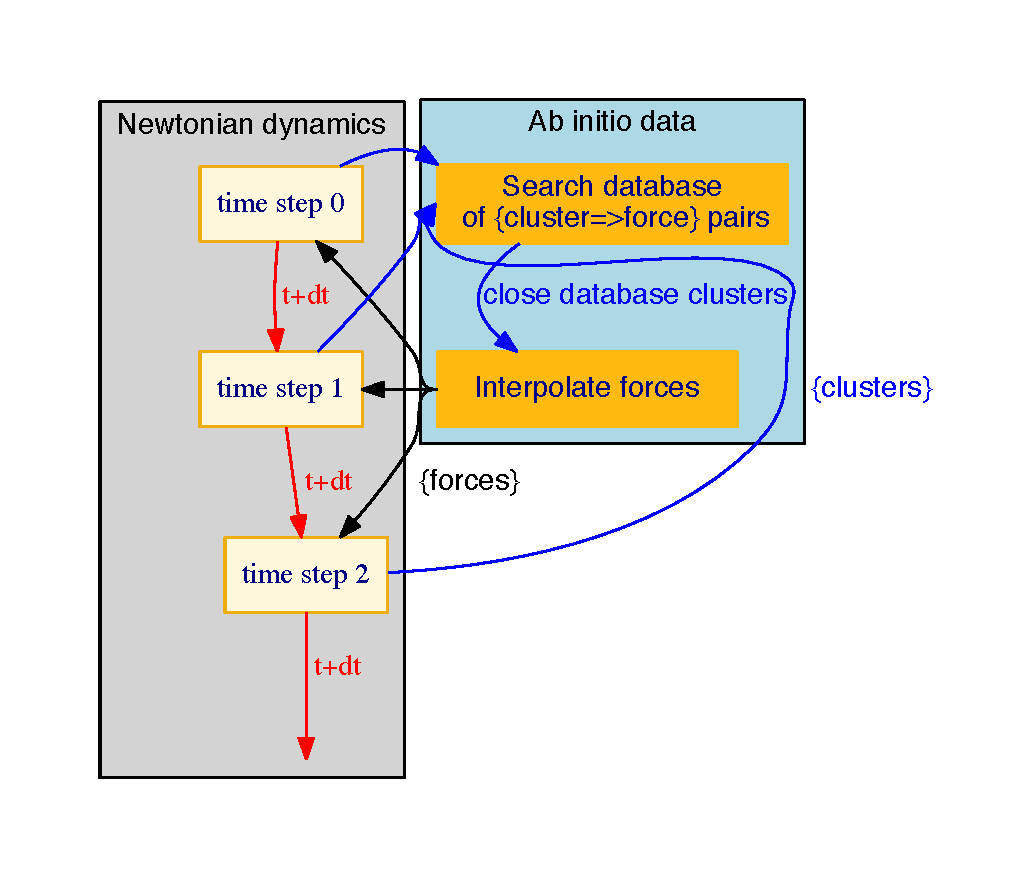
\includegraphics[width=\figwidth]{\figpath/algorithm.pdf}}
\caption{Schematic of the basic algorithm. The database search and force interpolation takes on the traditional role of an empirical potential.}
\label{fig:algorithm}
\end{figure}
%xxxxxxxxxxxxxxxxxxxxxxxxxxxxxxxxxxxxxxxxxxxxxxxxxxxxxxxxxxxxxxxxxxxxxxxxxxxx


Four questions will be answered in this work:
\begin{enumerate} [itemsep=0pt]
\item[Q1.] Does the force on the central atom in a neighborhood converge to that on the central atom of a corresponding sub-domain embedded in the full system?
\item[Q2.] Do the neighborhood-neighborhood distances directly correlate with the forces on the atoms in the clusters and how a large a neighborhood needs to be considered for the neighborhood-neighborhood comparison?
\item[Q3.] Is a database search fast enough to enable a feasible and efficient algorithm?
\item[Q4.] Is the error in the interpolation of forces controllable and convergent with increasing local density of samples in cluster space?
\end{enumerate}

Since the first question is directly related to the basic premise and is generally accepted, we will put it to rest here in the introduction.
(In fact the locality implied in question Q1 is the basic predicate of all empirical potentials.)
For traditional BO dynamics \cite{Marx2000,Kuhne2013}, the forces are derived from the Hellman-Feynman theorem, \ie from derivatives with respect to the nuclear coordinates of the energy formed from the electronic wave-functions.
Momentum is conserved because the forces are derived from this (implicit) potential dependent on all the nuclear positions; whereas, energy conservation is primarily due to the choice of time-integrator, as in classical MD.
Hence,
convergence of central force with neighborhood size implies conservation of momentum on par with BO dynamics.
As an illustration, a plot of the magnitude of the force $\| \fb(r) \|$ on atoms surrounding a perturbed atom as a function of distance from the perturbed atom $r$ is shown in \fref{fig:force_perturbation}a.
The samples obey the decay of force with distance
\begin{equation} \label{eq:force_scaling}
\| \fb(r) \| \le C \frac{\| \smallDelta \fb \|}{r^2}
\end{equation}
expected from Coulombic interactions, where $\smallDelta \fb$ is the force on displaced atom and the constant $C$ depends on the size of the perturbation.
Conversely, \fref{fig:force_perturbation}b shows that the force on the central atom of the system converges with the size of the isolated spherical sub-system relative to force calculated in the full periodic system.
These results give us confidence that for materials with a sufficiently large dielectric constant, only a limited number of nearest neighbors are needed to determine the force on a central atom.
When we use the proposed neighborhood decomposition in a large scale simulation, we lose the explicit dependence of the force on the coordinates of the atoms outside the neighborhood. 
The variation in the true, full-system force for neighborhoods in the database that are zero (cluster) distance apart is a measure of the error introduced by the cluster approximation. 
This phenomenon is explored further in the Results section.

%xxxxxxxxxxxxxxxxxxxxxxxxxxxxxxxxxxxxxxxxxxxxxxxxxxxxxxxxxxxxxxxxxxxxxxxxxxxx
\begin{figure}[h]
\centering
\subfigure[]
{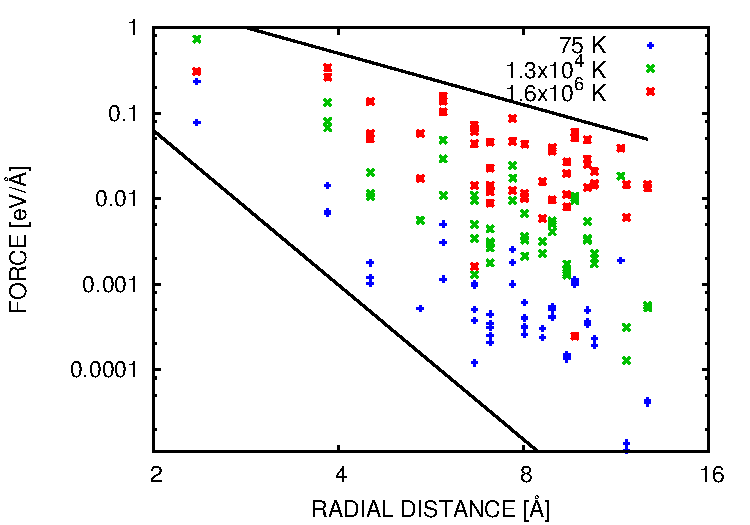
\includegraphics[width=1.02\figwidth]{\figpath/perturbation.pdf}}
\subfigure[]
{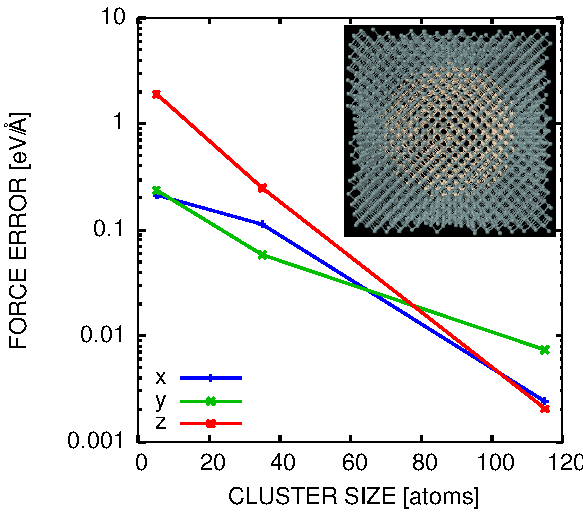
\includegraphics[width=0.8\figwidth]{\figpath/central_force_convergence.pdf}}
\caption{(a) Spatial decay of force due to a small perturbation in a perfect Si lattice as a function of the distance ($r$) from the perturbed atom.
The upper trend line is $\sfrac{1}{r^2}$, the lower is $\sfrac{1}{r^6}$ and the equivalent temperatures are estimated from the energy of the perturbation $\smallDelta E$ as $T \equiv \smallDelta E / k_B$.
(b) Convergence of the difference in forces on the central (perturbed) atom in an isolated cluster with increasing neighborhood size (in number of atoms) and in a fully periodic system.
(Inset) periodic 1000 atom system (cube containing blue and tan atoms) and sub-configuration (sphere containing tan atoms) with a perturbed central atom.  
}
\label{fig:force_perturbation}
\end{figure}
%xxxxxxxxxxxxxxxxxxxxxxxxxxxxxxxxxxxxxxxxxxxxxxxxxxxxxxxxxxxxxxxxxxxxxxxxxxxx

With regard to questions Q\,2-4, we need a metric to measure the distance between neighborhoods and thus their similarity.
There are many similarity measures proposed and in use for structure comparison and reconstruction \cite{Fogolari2012,Hung2012}, potential energy exploration \cite{Bartok_PhysRevB_2013,de2014relation} and the related field of sequence comparison \cite{Levitt1998,Baudet2012}, but not all are metrics and hence do not enable efficient geometric database queries.
We concentrate on two metrics: (a) the well-known \emph{Root Mean Squared Deviation} (RMS-D) and (b) our adaptation of the overlap of Gaussian type orbitals (OGTO) \cite{sadeghi2013metrics} and its spherical harmonic decomposition, the so-called \emph{Smooth Overlap of Atomic Positions} (SOAP) \cite{Bartok_PhysRevB_2013} measure. 
which is a spherical harmonic decomposition of the overlap of Gaussian type orbitals (OGTO) in \cref{sadeghi2013metrics}.
The RMS-D metric is commonly used in protein folding and drug discovery to quantify geometric similarity between molecules. \cite{Drineas2006,Hung2012,Carugo2007,Lindorff2009,Fogolari2012,sadeghi2013metrics}.
The origins of the SOAP representation trace to the \emph{bond-order} formalism \cite{Pettifor1989}.
\footnote{
Other measures include: 
(a) so-called \emph{fingerprint} differences between eigenvector representations of the symmetric matrix formed from interatomic distance of neighborhoods \cite{sadeghi2013metrics,de2014relation}  (\ie the spectral content of the edge distance-weighted adjacency matrix of graph theory \cite{vishveshwara2002protein,gutman1973graph}), 
(b) the Weyl matrix of inner products of position vectors \cite{Bartok_PhysRevB_2013},
(c) the Kullback-Leibler and Jensen-Shannon divergences of the probability density representations of the point densities \cite{Lindorff2009}, 
as well as (d) straightforward central moments of the point masses comprising the neighborhood configuration.
}

In the next section, \sref{sec:theory}, we will develop metrics to compare the similarity of a given local configuration and those stored in a database and then, based on this measure, interpolate the associated forces to give an estimate for the force on any given atom.
In \sref{sec:method} we will outline an algorithm to efficiently search through a large database of configuration-force pairs using the metric properties of the distance measure and a hierarchical graph representation of the database.
Then, in \sref{sec:results} in addition to testing the conservation properties of the algorithm, we address questions Q2-4 with results generated with the proposed method.
Finally, in \sref{sec:discussion} we conclude with a discussion of the results and ideas for future work.

%%%%%%%%%%%%%%%%%%%%%%%%%%%%%%%%%%%%%%%%%%%%%%%%%%%%%%%%%%%%%%%%%%%%%%%%%%%%%%
\section{Theory} \label{sec:theory}
%%%%%%%%%%%%%%%%%%%%%%%%%%%%%%%%%%%%%%%%%%%%%%%%%%%%%%%%%%%%%%%%%%%%%%%%%%%%%%
In this section we introduce the two chosen metrics, RMS-D and OGTO/SOAP, including means of determining the optimal rotation and permutation for appropriately invariant comparison of clusters. 
At the heart of both metrics is a representation of local atomic configuration.
Then we apply these metrics to the task of approximating the force on the central atom of given neighborhood by interpolation of forces of nearby neighborhoods with pre-computed forces.
These developments form the basis for database construction and search algorithms given in the following Methods section.

%=============================================================================
\subsection{Cluster distance metrics}
%=============================================================================
Given a configurational neighborhood $A$ of all atoms, $\alpha \in \Nc_A \equiv \{b_1\ldots b_{N_A}\}$, in a ball around a central atom $a$:
\begin{equation}
\neighborhood_A = \{ \xb_{\alpha_1 a}, \xb_{\alpha_2 a}, \xb_{\alpha_3 a}, \ldots, \xb_{\alpha_{N_A} a} \}
\end{equation}
where $\xb_{\alpha a} \equiv \xb_\alpha - \xb_a$ are distance vectors relative to the position of the central atom $\xb_a$,
the basic properties that a distance metric $d(A,B)$ between neighborhoods $A$ and $B$ must satisfy are:
\begin{enumerate} \setlength{\itemsep}{-10pt}
\item[M1.] {\bf coincidence}: $d(A,B) = 0 \ \text{if and only if} \ \neighborhood_A=\neighborhood_B $ 
\item[M2.] {\bf positivity}:  $d(A,B) > 0 $ 
\item[M3.] {\bf symmetry}:    $d(A,B) = d(B,A)$
\item[M4.] {\bf triangle inequality}: $d(A,C) \le d(A,B) + d(B,C)$ 
\item[M5.] {\bf reverse triangle inequality}: $d(A,C) \ge | d(A,B) - d(B,C) |$ 
\end{enumerate}
in addition to the physical invariances $d(A,B) = d(A,B')$:
\begin{enumerate} \setlength{\itemsep}{-10pt}
\item[I1.] {\bf translation}: $\neighborhood_B \to \neighborhood_{B'} = \neighborhood_B + \ab$
\item[I2.] {\bf rotation}:    $\neighborhood_B \to \neighborhood_{B'} = \Rs \neighborhood_B $
\item[I3.] {\bf permutation}: $\neighborhood_B \to \neighborhood_{B'} = \Ps \neighborhood_B $
\end{enumerate}
Note that the use of relative distances $\xb_{\alpha a}$ is a simple means of enforcing translational invariance; and, the reverse triangle inequality (M5) is an elementary  implication of the triangle inequality (M4).

With an inner product a distance metric can be generated directly.
In general, an inner product has three properties:
\begin{enumerate} \setlength{\itemsep}{-10pt}
\item[P1.] {\bf symmetry}: $\langle A, B \rangle = \langle B, A \rangle$
\item[P2.] {\bf linearity}: $\langle s A + B, C \rangle = s \langle A, C \rangle + \langle B, C \rangle$ 
\item[P3.] {\bf induction of a norm}: $\| A \|^2 \equiv \langle A, A \rangle \ge 0$ and $\langle A, A \rangle = 0$ only if $A = 0$
\end{enumerate}
the last of which induces a metric $d(A,B) = \| A - B \|$.

%=============================================================================
\subsubsection{RMS-D}
%=============================================================================
Assuming that the size of all clusters $N$ is the same  $N_A = N_B \equiv N$,
a weighted root mean square deviation (RMS-D) comparison metric is simply
\begin{equation} \label{eq:RMSD}
\begin{split}
d_\text{\tiny{RSMD}}(A,B) 
&= \min_{\Rb,\Ps} \sqrt{ \sum_{\alpha,\beta=1}^{N} \underbrace{ \|\xb_{\alpha a} -  \Rb \xb_{\beta b} \|^2}_{r^2_{\alpha\beta'}}  \ P_{\alpha\beta}  }   \\
&= \min_{\Rb,\Ps} \sqrt{ \left( \Xs_A - \Xs_B \Rb^T \right) \cdot \Ps \left( \Xs_A - \Xs_B \Rb^T \right) }
= \min_{\Rb,\Ps} \| \Xs_A - \Xs_B \Rb^T \|_\Ps  
 \\
&= \min_{\Rb,\Ps} \sqrt{ \|\Xs_A\|^2_\Ps + \|\Xs_B\|^2_\Ps - 2 \Xs_A \cdot \Ps \Xs_B \Rb^T } 
\end{split}
\end{equation}
where $\Xs_A =[ \xb_{\alpha_1 a}, \xb_{\alpha_2 a}, \xb_{\alpha_3 a}, \ldots, \xb_{\alpha_{N_A} a} ]^T$ and $\Xs_B$ are ($N\times 3$) matrices of the neighborhood vectors,
%\footnote{Note that the cluster matrices $\Xs_A$ and $\Xs_B$ can be seen as vectors embedded in a Euclidean space of dimension $3N$ with the usual inner product $\Xs_A \cdot \Xs_B$.  This space also represents a reduction of the dimensionality of the configurational space of the system from 3 times the number of atoms to 3 times the assumed size $N$ of the largest representative cluster.}
$\Rb \in \mathsf{SO(3)}$ is a (physical $3\times 3$) rotation of the neighborhood and $\Ps$ is a ($N\times N$) permutation of ordering of atoms in the neighborhood, \ie a binary orthogonal matrix which is simply the rearrangement of the rows of the identity matrix
\footnote{Regarding notation, a boldface font will be used for vectors and tensors in real space, \eg $\Rb$ and $\ab$; whereas, a sans-serif font will be employed for general matrices, \eg $\Ps$.}.
The permutation matrix $\Ps$ selects which of the pair-wise distances between atoms of the two configurations will contribute to the metric $d_\text{\tiny{RSMD}}$.

To determine the optimal rotation $\Rb$, Kabsch \cite{Kabsch1976} devised the following solution to this version of Wahba's problem \cite{Wahba1965}.
Starting with \eref{eq:RMSD} and noticing the last term is the only one dependent on $\Rb$ leads to:
\begin{equation} \label{eq:kabsch2}
2 \max_\Rb  \Xs_A \cdot \Ps \Xs_B \Rb^T
=
2 \max_\Rb  \tr \underbrace{\Xs_A^T \Ps \Xs_B}_{\Ub \Sb \Vb^T}  \Rb^T
=
2 \max_\Rb  \tr \Sb \Vb^T \Rb^T  \Ub 
= 2 \tr \Sb
\end{equation}
after application a singular value decomposition (SVD) of $ \Xs_A^T \Ps \Xs_B = \Ub \Sb \Vb^T $ where $\Ub,\Vb \in \mathsf{SO(3)}$ and $\Sb$ is diagonal and also of dimension 3. 
This term in the metric is maximized when $\Vb^T \Rb^T \Ub$ is the identity tensor and the resulting optimal rotation $\Rb = \Vb \Ub^T$ reduces the last term \eref{eq:RMSD} to the trace of the matrix of eigen-values $\tr \Sb$.
Consequently 
\begin{equation}
%d(A,B) = 
\min_{\Rb} \| \Xs_A - \Xs_B \Rb^T \|_\Ps  
=  \sqrt{ \|\Xs_A\|^2_\Ps + \|\Xs_B\|^2_\Ps - 2 \tr \Sb(\Ps) }
\end{equation}
for a fixed permutation $\Ps$
\footnote{The rotation $\Rb = \Ib$ maximizes since 
$\tr \Sb \Rb  = \tr \Rb \Sigma_i \lambda_i \eb_i \otimes \eb_i = \Sigma_i \lambda_i \Rb \eb_i \cdot \eb_i = \Sigma_i \lambda_i \Ib \eb_i \cdot \eb_i = \Sigma_i \lambda_i$, using an eigenvalue representation of $\Sb$.  Alternatives to the SVD-based solution exist most notably quaternion-based solutions \cite{Liu2010,sadeghi2013metrics}.}.

It remains to solve the permutation problem, \ie an optimal match is possibly only one of the $N!$ permutations of the ordering of the labels $\{1,2,\ldots,N\}$ for neighborhood $B$, which is clearly not independent of the optimization with respect rotation. 
This is a complex problem, as recognized in this and related fields, see \eg \cref{Baudet2012} and, in general, most applicable integer optimization methods are known to have difficulties with symmetries.
Possible solutions include using combinatorial programming algorithms like \emph{branch-and-bound} \cite{Hong2007,sadeghi2013metrics}.

Given the geometry of our application, our approach is to segregate the permutation problem into smaller sub-problems involving only the sets that have (nearly) identical radial sorts, \ie equivalent shells. 
As an alternative to this straight-forward $r$-sort and permute, we can use the spectral representation of the clusters to perform what we call a $\lambda$-sort:
\begin{enumerate} \setlength{\itemsep}{-10pt}
\item Form the adjacency matrices $[\As]_{ij} = r^2_{\alpha_i\alpha_j} $ for both $A$ and $B$ and compute eigen-system for $\As_A$ and $\As_B$
\item Compare the eigenvalues $\lambda_i$ of $\As_A$ and $\As_B$, starting with the largest. 
If $\lambda_i^A \approx \lambda_i^B$ then sort and match the components of the corresponding eigenvectors $\eb_i^A$ and $\eb_i^B$ to form a order map $m: a \in Q \to  b \in B$ and hence a trial permutation matrix $\Pb_{a,m(a)} = 1, \ \forall a \in Q$. 
\end{enumerate}
In preliminary tests the $\lambda$ sort, albeit more expensive, succeeded in finding the best match cases where the $r$-sort failed \eg a tetrahedral arrangement of neighbors with only one atom perturbed.
In any event the overall method does not require the optimal match in all queries if the database is dense and perhaps redundant with permutations of a given configurations.

Lastly, the assumption of locality motivates the use of a weighted norm within the radial cutoff implicit in the chosen cluster size.
We can set the non-zero entries of of the permutation operator $P_{\alpha\beta}$ to the value of positive weight function dependent on the radial coordinates of $\alpha$ and $\beta$ 
so that the distance metric is less sensitive to neighbors far away from the central atom.
Also the usual normalization by number of atoms, $1/(N+1)$, can be accommodated in $\Ps$ which creates an interpretation of $d$ as an average atom-to-atom distance.
As proved in \cref{Steipe2002} via equivalence classes induced by the optimal rotation, the RMS-D measure is a valid distance metric.

%=========================================================================
\subsubsection{OGTO}
%=========================================================================

As we will see, the so-called overlap of Gaussian type orbitals (OGTO) is more complex than RMS-D; however, it has the advantage of being intrinsically permutationally invariant by comparing all atom locations in one cluster to those in the other in a weighted fashion (instead of specific pairs with RMS-D).
OGTO starts with the representation of atomic density of a neighborhood surrounding a central atom (whose density, $\Delta(\mathbf{0})$, we omit in the representation, as in the RMS-D metric):
\begin{equation} \label{eq:sph_harm_expansion}
\rho_A(\xb) = 
\sum_{\alpha\in\Nc_A} \Delta(\xb_{\alpha  a}) 
\end{equation}
in terms of Gaussian smeared point densities 
\begin{equation}
 \Delta(\xb) = \frac{1}{(\sqrt{2 \pi} \sigma)^{3}} \exp\left(- \frac{ \| \xb \|^2}{2\sigma^2}\right) ,
\end{equation}
with width $\sigma$
\footnote{The smearing $\sigma$ could be assigned in a per-atom/element fashion for greater specificity.}.
With this representation, we can form the product 
between the atomic densities of neighborhoods $A$ and $B$:
\begin{equation} \label{eq:ogto_inner_product}
\begin{split}
\left<\rho_A,\rho_B\right> &= \int \mathrm{d}\xb \,  \rho_A(\xb) \rho_B(\xb)
=  \int \mathrm{d}\xb \, \sum_{\alpha\in\Nc_A} \Delta(\xb-\xb_\alpha) \sum_{\beta\in\Nc_B} \Delta(\xb-\xb_\beta) \\
&= \sum_{\alpha \in \Nc_A,\beta \in \Nc_B}  \int \mathrm{d}\xb \, \Delta(\xb-\xb_\alpha) \Delta(\xb-\xb_\beta)  \\
&= \frac{1}{(2 \sqrt{\pi} \sigma)^3} \sum_{\alpha\in\Nc_A,\beta\in\Nc_B} \exp\left( -\frac{r_{\alpha\beta}^2}{4 \sigma^2} \right)
\end{split}
\end{equation}
and thenceforth, an OGTO-based metric: 
\begin{equation} \label{eq:ogto_norm}
\begin{split}
&d_\text{\tiny{OGTO}}(A,B)  
= \min_\Rb \sqrt{ \left<\rho_A, \rho_A\right> + \left<\rho_B,\rho_B\right> - 2 \left<\rho_A,\Rb \rho_B\right>} \\
&= \frac{1}{(2 \sqrt{\pi} \sigma)^{\frac{3}{2}}} \sqrt{
\sum_{\alpha_1,\alpha_2\in\Nc_A}  \exp\left( -\frac{r_{\alpha_1\alpha_2}^2}{4 \sigma^2} \right)
+
\sum_{\beta_1,\beta_2\in\Nc_B}    \exp\left( -\frac{r_{\beta_1\beta_2}^2}{4 \sigma^2} \right)
-2 \min_\Rb
\sum_{\alpha\in\Nc_A,\beta\in\Nc_B}       \exp\left( -\frac{r_{\alpha\beta'}^2}{4 \sigma^2} \right)
} 
\end{split}
\end{equation}
where $r^2_{\alpha\beta'} = \|\xb_\alpha - \Rb \xb_\beta\|^2$ as in \eref{eq:RMSD}.
(Clearly, this product \eqref{eq:ogto_inner_product} is non-negative given positive densities but given its form does not satisfy the linearity requirement, P2, of a true inner product.)

The rotationally dependent term can be expressed in terms of \emph{Wigner D matrices} \cite{BiedenharnLouck} $\Ds_l = \Ds_l(\Rb)$ 
%\footnote{$\Ds_l(\Ib)$ is a ${2l+1}$ identity matrix.}
\begin{equation}
\left<\rho_A,\Rb \rho_B\right> 
= \sum_{l=0}^\infty \tr \Ds_l(\Rb) \Js_l
\approx \underbrace{\tr \Ds_0(\Rb) \Js_0}_{\Js_0}  + \tr \Ds_1(\Rb) \Js_1
\end{equation}
and corresponding rotationally independent terms $\Js_l$ based on the representation of (smeared) atomic densities in SOAP which we use as a convenient decomposition of the Gaussian overlap \eref{eq:ogto_inner_product}, see \aref{app:soap} for more details.
Since  $\Ds_0 = 1 $ is constant and the dimensions of $\Ds_1$ are the same as $\Rb$ albeit being complex valued, 
we can find the optimal rotation $\Rb$ that maximizes the inner product $\left<\rho_A,\Rb \rho_B \right>$ 
\begin{equation} \label{eq:D_expansion}
\argmax_\Rb \left<\rho_A,\Rb \rho_B\right>  =
\argmax_\Rb \sum_{l=0}^p \tr \Js_p \Ds_p(\Rb) 
%\ \ \longrightarrow \ \ 
\approx \argmax_\Rb \tr \Js_1 \Ds_1(\Rb)
\end{equation}
using an SVD of the matrix $\Js_1$ in a manner analogous the solution for the optimal rotation of the RMS-D metric.
First, we apply the mapping $ \Ds_1 = \As^\dagger \Rb \As $ from \cref{BiedenharnLouck} (Eq. 3.63): 
\begin{equation}
\tr \Js_1 \Ds_1
= \tr \Js_1 \As^\dagger \Rb \As  
= \tr \underbrace{ \As \Js_1 \As^\dagger }_{\Ub \Sb \Vb^T} \Rb
\end{equation}
where the transformation matrix $\As: \Ds \rightarrow \Rb = \As \Ds \As^*$ is constant and unitary.
Hence, the optimal (real-valued) rotation is $\Rb = \Vb \Ub^T$.
Unfortunately the truncated sum in \eref{eq:D_expansion} does not encode all the configurational information, and hence we use it as an initial guess to a Newton solver based on the derivative 
\begin{equation}
\frac{\partial}{\partial \Rb} d_\text{OGTO}(A,B) =  -\frac{2 \sigma \sqrt{\pi}^3}{d_\text{OGTO}(A,B)} \sum_{\alpha\in\Nc_A,\beta\in\Nc_B} \exp\left( -\frac{r_{\alpha\beta'}^2}{4 \sigma^2} \right)  \xb_\alpha \otimes \xb_\beta
\end{equation}

Given the fact that the interatomic distances $r_{\alpha\beta}$ appear in an exponential function in \eref{eq:ogto_inner_product}, this product does not satisfy the linear property (P2) of true inner products. 
Nevertheless, \eref{eq:ogto_norm} appears to satisfy the properties of a metric (M1-5).
As an illustration, \fref{fig:soap} shows, for a range of values of $\sigma$ on order of atomic spacing, that both the OGTO and RMS-D metrics satisfy the triangle inequality (M4) for the distances between a two arbitrary configurations $\neighborhood_1$, $\neighborhood_2$,  and a third $\neighborhood_3$ which is interpolation of the two: $\Xs_3 = \alpha \Xs_1 + (1-\alpha) \Xs_2$.
The RMS-D metric shows the expected linearity with $\alpha$: $d_{13} = (1-\alpha) d_{12}$ and $d_{23} = \alpha \, d_{12}$
\footnote{ For RMS-D, the fact that $r^2_{13} = || \xb_1 - (\alpha \xb_1 + (1-\alpha) \xb_2) ||^2  = (1-\alpha)^2 r^2_{12}$ and $r^2_{23} = || \xb_2 - (\alpha \xb_1 + (1-\alpha) \xb_2) ||^2  = \alpha^2 r^2_{12}$ for every atom pair leads to the linearity shown.  },
 whereas the OGTO distances only regresses to this behavior with larger $\sigma$.
Unfortunately, this asymptotic satisfaction of condition P2 comes with decreasing discrimination of close atom pairs, since all $r^2_{\alpha\beta}$ become weighed equally as $\sigma$ is increased. 
Nevertheless, for any given atomic system a range of suitable $\sigma$ is easy to find.

%xxxxxxxxxxxxxxxxxxxxxxxxxxxxxxxxxxxxxxxxxxxxxxxxxxxxxxxxxxxxxxxxxxxxxxx
\begin{figure}[h]
{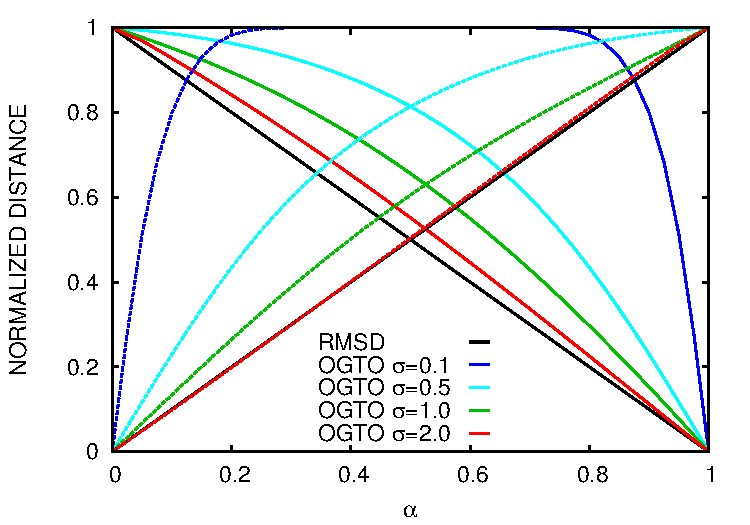
\includegraphics[width=\figwidth]{\figpath/triangle_test.pdf}}
\caption{Demonstration of the triangle inequality (M4) and illustration of OGTO distance sensitivity to width of smearing function $\sigma$.
Distances shown are from $\neighborhood_3: \Xs_3 = \alpha \Xs_1 + (1-\alpha) \Xs_2$ to $\neighborhood_1$ (dashed) and $\neighborhood_2$ (solid).
} \label{fig:soap}
\end{figure}
%xxxxxxxxxxxxxxxxxxxxxxxxxxxxxxxxxxxxxxxxxxxxxxxxxxxxxxxxxxxxxxxxxxxxxxx

%=========================================================================
\subsection{Interpolation} \label{sec:interpolation}
%=========================================================================

Given a viable metric $d_{QA} = d(Q,A)$, all the neighborhoods $\Bc_Q = \{ A \ | \ d_{QA} \le R \}$  within a ball $\Ball_Q$ around a query neighborhood $\neighborhood_Q$ can be found (via the search algorithm described in \sref{sec:metric_search}).
The forces on the central atoms of these nearby neighborhoods can be interpolated.
Radial basis functions (RBF) \cite{Buhmann2003} are a general class of functions amenable to this task.
We choose the inverse quadratic form
\begin{equation} \label{eq:rbf}
\phi(d) = \frac{1}{1+(\varsigma d)^2}
\end{equation}
motivated by the expected force decay in real space and choose the parameter $\varsigma \ll \sfrac{1}{R}$ based on the size of the trust region $\Bc_Q$.
Then,
to construct the interpolation solely based on the inter-cluster distances $d_{QB}$ and the neighboring forces $\fb_B$, we solve the consistency equations
\begin{equation} \label{eq:force_interpolation}
\Rb_{QA} \fb_A = \sum_{B\in \Ball_Q} \phi(d_{AB}) \, \ab_B  \ \text{for every} \ A  \in \Bc_Q
\end{equation}
for the coefficients $\{\ab_B\}$.
Here, the matrix $\phi(d_{AB})$ is symmetric and positive definite (where $d_{AB}$ is the edge-weighted \emph{adjacency} matrix of the sub-graph in the ball around $Q$ in cluster space), and $\Rb_{QA}$ is the optimal rotation from reference neighborhood $A$ to query neighborhood $Q$ which aligns the neighboring forces $\fb_A$ to the orientation of the cluster $Q$.
The local interpolation of the databased HF forces 
\begin{equation}
\fb_Q = \sum_{B\in \Ball_Q} \phi(d_{QB}) \, \ab_B 
\end{equation}
results.
%\footnote{Note that in this simple version the interpolant $\phi(d)$ does not satisfy the normalization condition  $\Sigma_B \phi(d_{QB}) = 1$.}.

%%%%%%%%%%%%%%%%%%%%%%%%%%%%%%%%%%%%%%%%%%%%%%%%%%%%%%%%%%%%%%%%%%%%%%%%%%
\section{Method} \label{sec:method}
%%%%%%%%%%%%%%%%%%%%%%%%%%%%%%%%%%%%%%%%%%%%%%%%%%%%%%%%%%%%%%%%%%%%%%%%%%

Beyond the basic theoretical developments there are a few more pragmatic components of the overall paradigm. 
Specifically, how to construct a viable dataset and an efficient search.

%=========================================================================
\subsection{Database generation} \label{sec:database}
%=========================================================================

The database is in effect a discrete representation/sampling of neighborhood configurational space as a graph with edges weighted by neighborhood-neighborhood distances.
Specifically, given a set of $M$ neighborhoods $\{\neighborhood_A, \ A = 1,\ldots M\}$, an atlas in the form of a complete edge-weighted graph: $\{d(A,B) \ | \ \forall  A,B\in \{ 1, \ldots M \}, A \neq B \}$, where the  $\sfrac{1}{2} \, M (M-1)$ edges represent the inter-cluster distances, can be generated.
%\footnote{In addition to inter-neighborhood distances, components of either metric can be {\it pre-computed} and stored: $\Xs_A$ for RMS-D and $\Ys_A$ for SOAP of cross term and the norms $|| \rho_A ||^2$. }.
For this work we generated samplings of cluster space by post-processing standard BO simulations of the dynamics of feasibly-sized periodic systems to extract HF forces and atomic neighborhoods
\footnote{Alternately, we also generated configurations with (a) a random walk, via a Monte Carlo algorithm, and (b) a classical MD surrogate of the system of interest.}.

Since a na\"{\i}ve graph that includes all possible edges would grow like the square of the number of stored clusters, we chose an $n$-level hierarchical representation where each level spans/covers a sub-graph, with the top-most level being the whole graph.
This representation, which maintains a fixed bandwidth adjacency matrix, is constructed via an algorithm based on $k$-medoids clustering \cite{kaufman1987clustering}:
\begin{enumerate} 
\item Group graph containing $\{\neighborhood_A\}$ using $k$-means based on distance
\begin{enumerate}
\item initialize by randomly picking $k$ candidate medoids $\{\neighborhood_{A_i}, \ i=1,k \}$ 
\item assign each $\neighborhood_B$ to group $\Gc_i^n$ based on closest medoid $\neighborhood_{A_i} = \underset{A_i\in\Gc_i^n}\argmin \, d(A_i,B)$
\item update medoids $\{\neighborhood_{A_i}, i=1,k\}$ by ${A_i} = \underset{A_i\in\Gc_i}\argmin \displaystyle\sum_{B\in\Gc_i^n} d(A_i,B)$
\item repeat (b) and (c) until groups $\{ \Gc_i^n, \, i=1,k \}$ do not change 
\end{enumerate}
\item For each group $\Gc_i$, select medoid $A_i \in \Gc_i^n$  as the representative reference for this sub-graph at this level.
\item Repeat for each sub-graph containing $\Gc_i^n$ until each sub-graph of the current level $n$ is of most size $k$.
\end{enumerate}
Note that each level is fully connected, \ie all edges for the sub-graph are stored, so that metric search described in the next section will converge.
Also, at the lowest level each neighborhood $\neighborhood_A$, in addition to being connected to all other neighborhoods on its level, is connected to all close neighborhoods within a radius twice that of the interpolation trust ball $\Bc_A$ to ensure the force interpolation described in \sref{sec:interpolation} captures all local clusters.
So, at the lowest level the groupings $\Gc_i$ form an overlapping cover of the whole set and this is the primary difference with the {\it ball tree} search in the machine learning literature \cite{weinberger2009distance}.

In general, the chemical composition of the neighborhoods segregate the database into separate/disjoint spaces and hence herein we treat a single species for simplicity.
It should be noted that the configurational space visited by dynamics will typically be bounded by energy or temperature and hence the database samples will be dense in some region of configuration space.
Also, the symmetries I1-I3 will tend to compact the database into a sub-manifold of the basic $\Rbb^{3N}$ cluster space by creating equivalence classes \cite{Steipe2002}, \eg setting the central atom at the origin removes the translational ambiguity, the optimal rotation reduces the dimensionality by another 3 dimensions, and optimal permutations condense segregated, equivalent high symmetry neighborhoods into dense groupings.
Ultimately, the density of configuration-force samples determines the accuracy of the force interpolation that drives the dynamics.
Appropriate adaption alleviates concerns about having an dense sampling from the outset but here we treat the task of pre-computing a static database (one that could be used as an initial database for an adapting method).
More ideas regarding this issue will be discussed in the concluding section.


%=========================================================================
\subsection{Metric-based search} \label{sec:metric_search}
%=========================================================================

Recent work \cite{Fogolari2012} has shown that an atlas of precomputed distances can accelerate molecular structure searches by orders of magnitude versus a simple exhaustive search of a configurational database.
The associated algorithm relies on the reverse triangle inequality (M5) which implies that the distances between two pairs $(Q,A)$ and $(A,B)$ with an element $A$ in common puts bounds on the distance $d(Q,B)$.  
In fact, given $d(A,B) > 2d(Q,A)$ and M5, $d(Q,B) \ge |d(A,B)-d(Q,A)|$, then $d(Q,B) > |2d(Q,A)-d(Q,A)| = d(Q,A)$.
If $Q$ is a query cluster this fact allows the search to omit all clusters $\{ B \ | \ d(A,B) > 2d(Q,A)\}$, using the distances $d(A,B)$ stored in the database and the newly computed distance $d(Q,A)$.

A version of this metric-based search algorithm adapted from \cref{Fogolari2012} to our hierarchical database is:
\begin{enumerate}[itemsep=-5pt]
\item Given a query cluster $Q$, initialize $d_\text{min} = d(Q,A_\text{min})$ where $A_\text{min}$ is the first element in $\mathcal{G}^0$, the set of all configurations in the highest level $n=0$ 
\item For each level $n$ find $A_\text{min}^n = \underset{A \in \mathcal{G}_i^n}{\argmin} \, d(Q,A)$ via iteration over $A \in \Gc = \Gc_i^n$:
\begin{enumerate}[itemsep=-5pt]
\item compute $d = d(Q,A)$
\item if $d < d_\text{min}$, set $A_\text{min} = A$, $d_\text{min} = d$ and, using the sorted distances stored in the database, update $\Gc = \{ B \, | \, d(A_\text{min},B) < 2 d_\text{min} \}$
\item if $\Gc$ contains only $A_\text{min}$, move to the next lowest level. 
\end{enumerate}
\item If at the lowest level, search over the region of radius $2 R$ around $A_\text{min}$ to obtain  $\Bc = \{ A_j \ | \ d(Q,A_j) < R\}$
\item Store set $\Bc$ for subsequent searches for the atom associated with $Q$.
\end{enumerate}
and is illustrated in \fref{fig:search}.
A proof of convergence to the optimal $A_\text{min}$ and the group around it can be constructed along the lines of convergence of sequence in a complete metric space: the graph is complete and the candidate $A_\text{min}$ moves closer to the optimal $A_\text{min}$ with iteration.
With regard to the last step of the algorithm, unlike the task of matching molecules and chemical compounds by structure, with dynamics we have history and continuity in time and the assumption that in a small time-step $\dt$ the particular cluster of interest has not moved very far through cluster space.
So at time $t+\dt $ rather than searching over the entire space of neighborhoods, we will begin the search in the ball about the best match for the previous time $t$. 

%xxxxxxxxxxxxxxxxxxxxxxxxxxxxxxxxxxxxxxxxxxxxxxxxxxxxxxxxxxxxxxxxxxxxxxxx
\begin{figure}[h]
{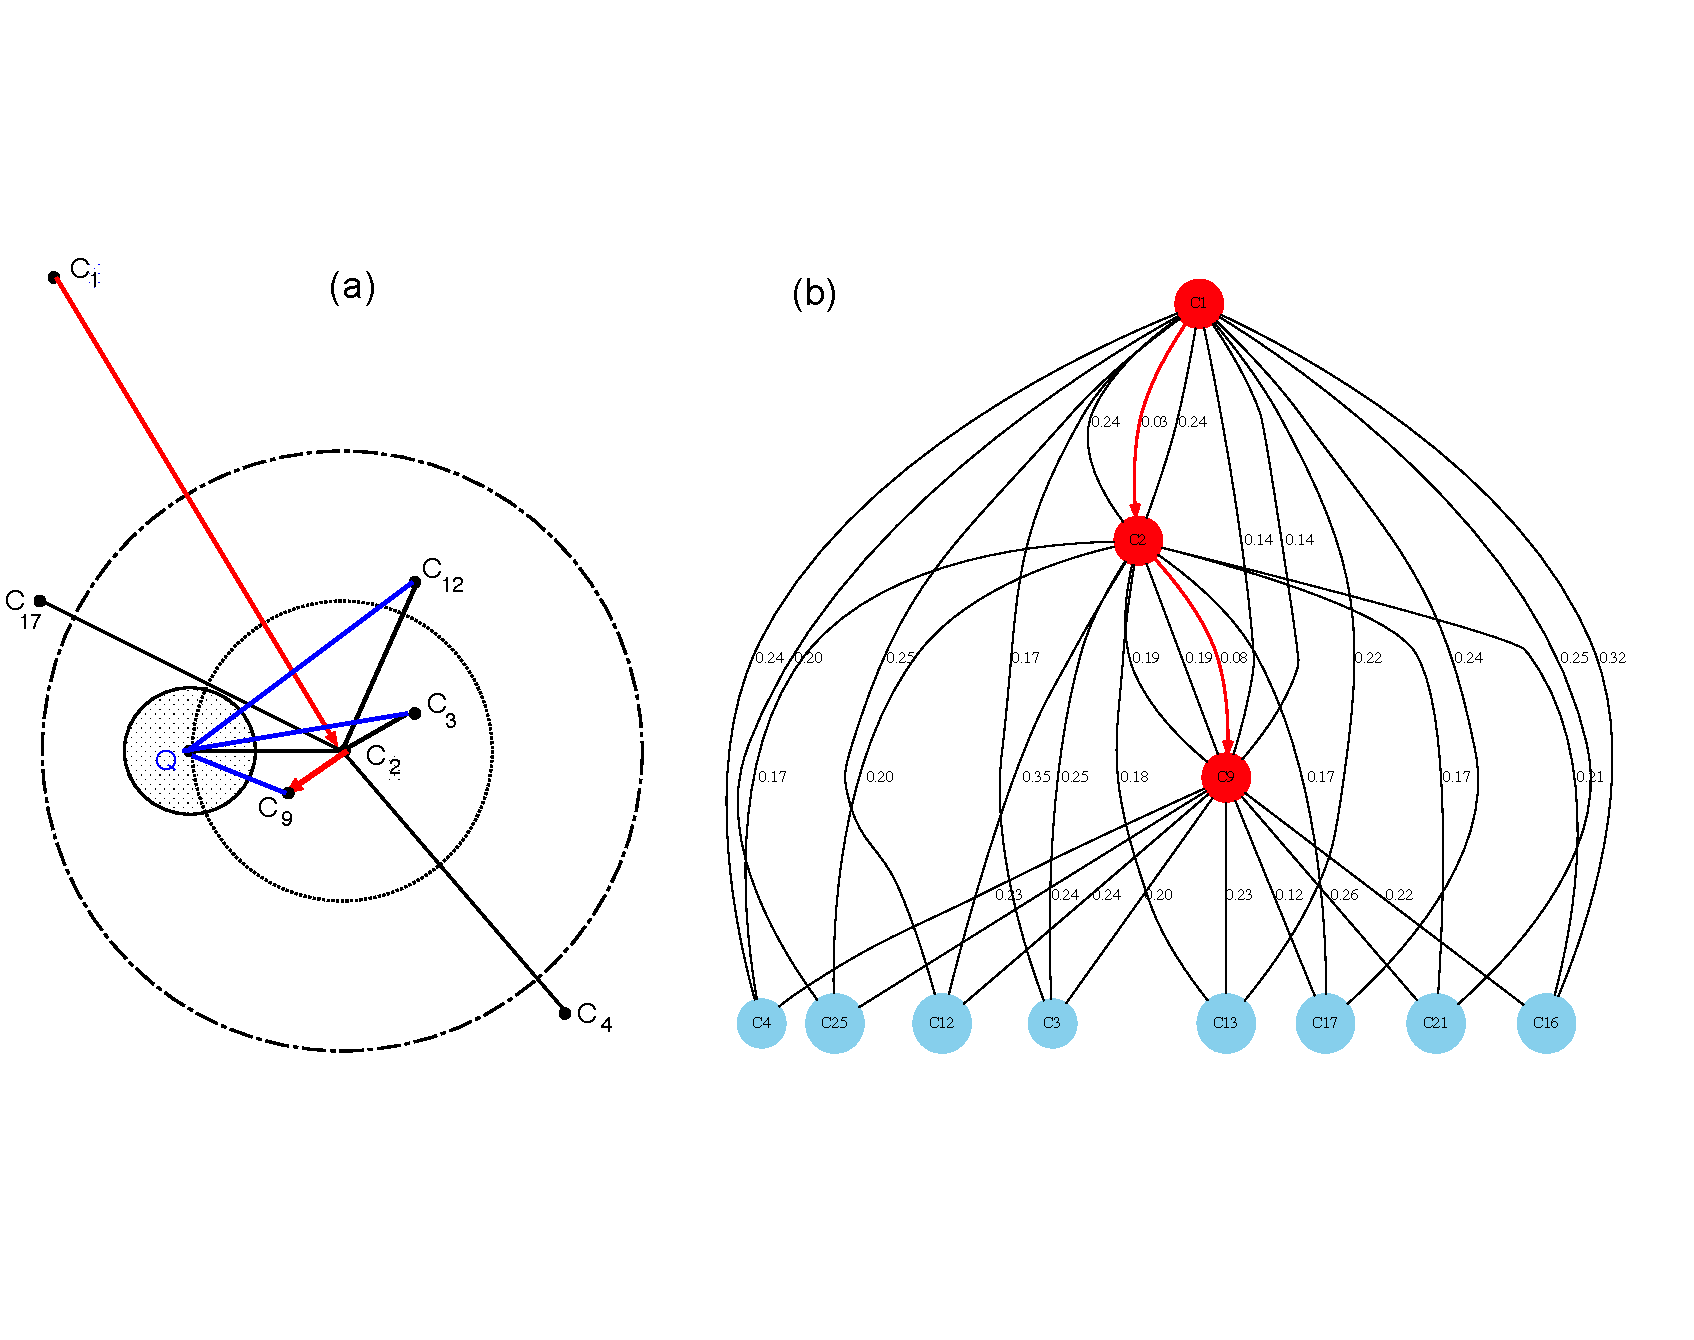
\includegraphics[width=1.9\figwidth]{\figpath/metric_search-combined.pdf}}
\caption{
Metric search algorithm:
(a) Illustration of metric search for query point Q.
Given a current closest cluster, say, $\neighborhood_2$, the subset \{  $\neighborhood_3$, $\neighborhood_9$, $\neighborhood_{12}$ \} near $\neighborhood_2$ are intermediate candidates for inclusion in the (shaded) interpolation ball around Q; whereas, the other neighbors, $\neighborhood_i$, of $\neighborhood_2$, $\neighborhood_3$ $\neighborhood_9$, can be ignored since $d(\neighborhood_i,\neighborhood_2) > 2 d(Q,\neighborhood_2)$.
After direct computation of distances from the candidate subset to Q in the next search iteration, $\neighborhood_9$ will be selected as the new closest configuration to Q.
The distances that need to be computed are shown in blue, the distances that are retrieved from the database are in black and the search path connecting successive closest stored configurations is shown in red.
(b) The corresponding search path through a portion of the database visualized as a graph.
}
\label{fig:search}
\end{figure}
%xxxxxxxxxxxxxxxxxxxxxxxxxxxxxxxxxxxxxxxxxxxxxxxxxxxxxxxxxxxxxxxxxxxxxxxx
 

%%%%%%%%%%%%%%%%%%%%%%%%%%%%%%%%%%%%%%%%%%%%%%%%%%%%%%%%%%%%%%%%%%%%%%%%%%%%%%
\section{Results} \label{sec:results}
%%%%%%%%%%%%%%%%%%%%%%%%%%%%%%%%%%%%%%%%%%%%%%%%%%%%%%%%%%%%%%%%%%%%%%%%%%%%%%

All the following results use two samples of the \abinitio dynamics of a Si system, one crystalline at 300 K  and the other amorphous at 2500K. 
The sampled system is periodic with 216 atoms (4$^3$ unit cells) and sampled for 200-1000 steps of 1 fs with the first 100 steps discarded since the starting state was a perfect crystal.
Given that the first shell of the diamond cubic structure has 4 neighbors and the second 12 neighbors, we choose clusters with 4 and 16 neighbors.


As a preliminary to examining questions Q2-4, we examined sensitivities to algorithmic parameters.
Given the results shown in \fref{fig:soap}, for all the following studies we used the OGTO smearing parameter  $\sigma = 1 $\AA \ in $d_\text{OGTO}$.
For the scale parameter $\varsigma$ of the RBF used in the force interpolation \eref{eq:rbf} we used $\varsigma = 1 $\AA \ so that the RBF is sufficiently peaked in the interpolation ball (whose radius is on the order 2-4 \AA).
% Nearest & second nearest neighbor distances:sqrt(3.0)/4.0*a, sqrt(2.0)/2.0*a
Also, since $\lambda$-sort modification of the RMS-D metric is not a perfect solution to the permutation optimization we only used the less computationally expensive $r$-sort in our demonstrations.

Here we also examine the behavior of the two chosen metrics over the database of clusters provided by the BO trajectories.
\fref{fig:dynamics_path} is an illustration that the BO dynamics path in cluster space is continuous.
The bell shaped distributions of cluster RMS-D distances relative to a perfect lattice configuration broaden and shift to greater distances with increasing temperatures, as expected.
The increase in number of neighbors from 4 to 16 increases the specificity of the metric as evidenced by the relatively sharper distributions for distances based on $N=16$.
\fref{fig:spatial_vs_cluster}a shows the characteristic radial distributions for a crystalline material at 300K and an amorphous material at 2500K.
In \fref{fig:spatial_vs_cluster}b we compare the distribution of distances as a function of temperature and number of neighbors for both the RMS-D and OGTO measures for the whole database of configuration samples (as opposed to following the configuration associated with one atom through time, as in the inset of \fref{fig:dynamics_path}).
Although quantitatively different, the distributions generated by both metrics show peaks that are closer to zero distance for colder systems and fewer neighboring atoms in the cluster comparisons.


%xxxxxxxxxxxxxxxxxxxxxxxxxxxxxxxxxxxxxxxxxxxxxxxxxxxxxxxxxxxxxxxxxxxxxxxxxxxx
\begin{figure}[h]
{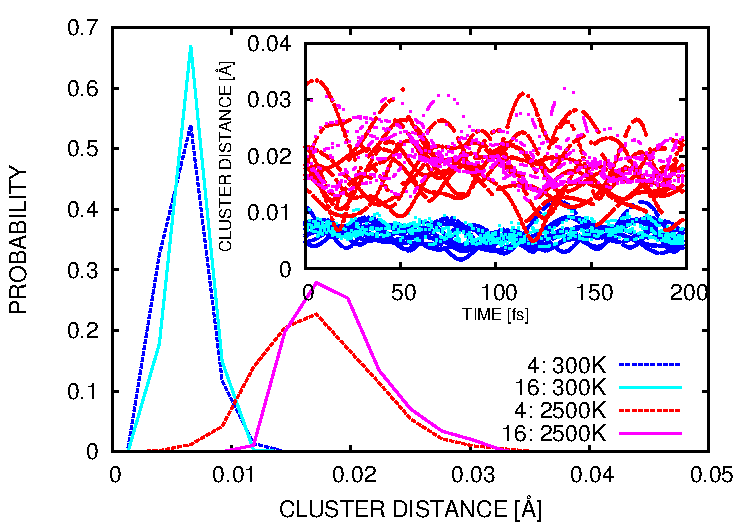
\includegraphics[width=\figwidth]{\figpath/path_distribution.pdf}}
\caption{Dynamics path (inset) and associated distance distribution of a single neighborhood through cluster space, where the (RMS-D) distance is measured from a perfect crystalline configuration.}
\label{fig:dynamics_path}
\end{figure}
%xxxxxxxxxxxxxxxxxxxxxxxxxxxxxxxxxxxxxxxxxxxxxxxxxxxxxxxxxxxxxxxxxxxxxxxxxxxx
\begin{figure}[h]
\subfigure[\ radial distribution]
{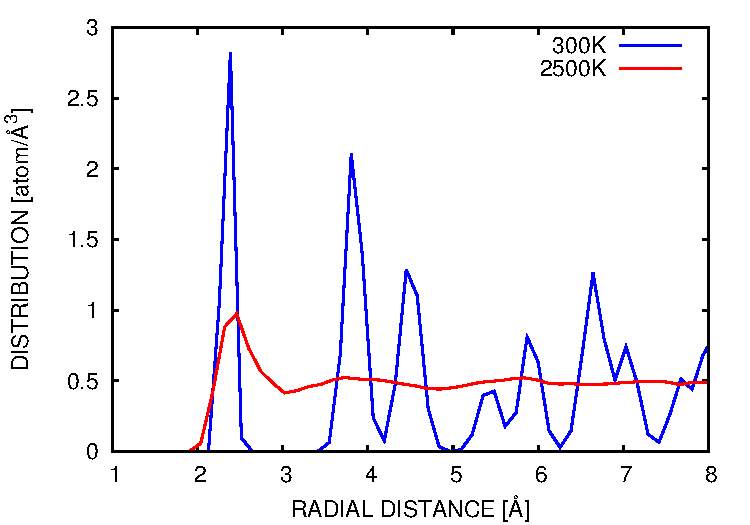
\includegraphics[width=\figwidth]{\figpath/rdf.pdf}}
\subfigure[\ histogram of inter-cluster distances]
{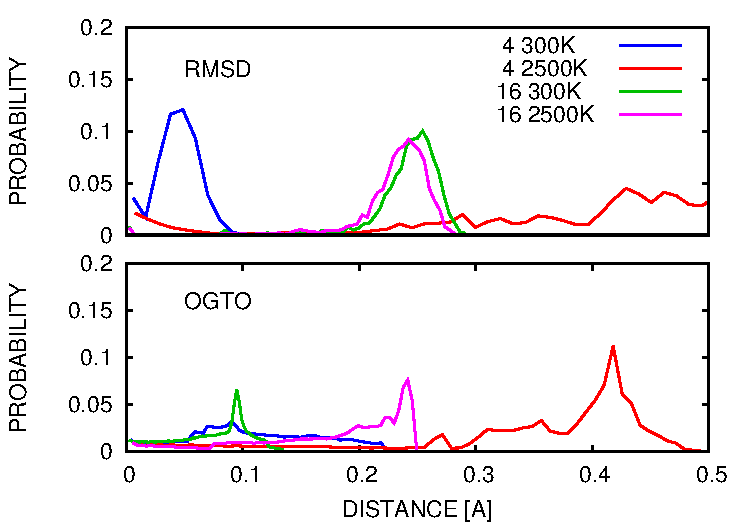
\includegraphics[width=\figwidth]{\figpath/distribution.pdf}}
\caption{
Spatial structure compared to cluster space structure.
(a) the radial distribution of Si at 300 K (crystalline) and 2500 K (melt).
(b) the distribution of pair-distances in the corresponding cluster space.
}
\label{fig:spatial_vs_cluster}
\end{figure}
%xxxxxxxxxxxxxxxxxxxxxxxxxxxxxxxxxxxxxxxxxxxxxxxxxxxxxxxxxxxxxxxxxxxxxxx

%===========================================================================
\subsection{Force-distance correlation}
%===========================================================================
In this section we address Q2 posed in the introduction:
one of the fundamental assumptions of the method is that the cluster distance between a pair of configurations is correlated with the similarity in the forces
\begin{equation}
\| \fb_A - \Rb_{AB} \fb_B \| \propto d_{AB}
\end{equation}
The force error \vs cluster distance correlation, \fref{fig:fvsd}, clearly shows that the HF forces and cluster distances are correlated and in fact that as $d\to 0$ the forces become effectively identical up to a rotation $\Rb_{AB}$. 
Also, as expected, using a larger number of atomic neighbors in a given cluster is more discriminating in terms of force errors and there is more scatter in the higher temperature results.
Lastly, it appears that the OGTO samples are denser and more linearly correlated with distance than those of the RMS-D over the same range of force error. 
In part this is likely due to the permutation mismatches in our implementation of RMS-D which leads to a density of low force error samples appearing at large cluster-cluster distances (not shown in \fref{fig:fvsd}a).


%xxxxxxxxxxxxxxxxxxxxxxxxxxxxxxxxxxxxxxxxxxxxxxxxxxxxxxxxxxxxxxxxxxxxxxxxxxx
\begin{figure}[h]
\subfigure[\ RMS-D]
{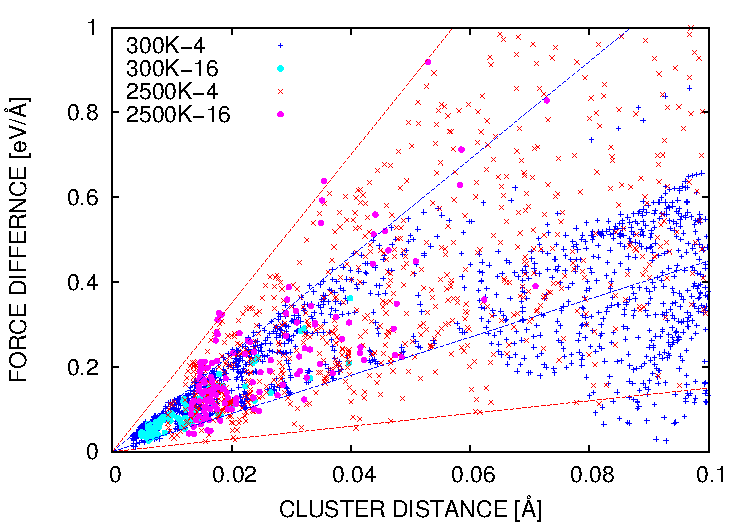
\includegraphics[width=\figwidth]{\figpath/RMSD_force-distance_correlation.pdf}}
\subfigure[\ OGTO]
{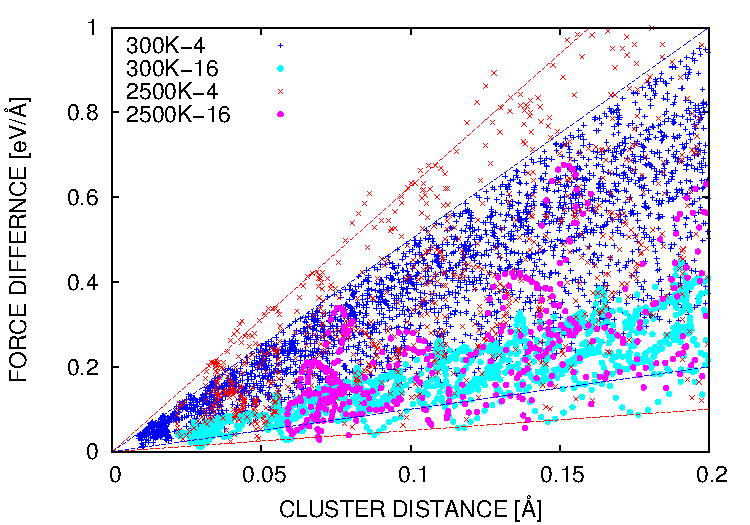
\includegraphics[width=\figwidth]{\figpath/OGTO_force-distance_correlation.pdf}}
{}
\caption{Force error-cluster distance correlation for (a) RMS-D and (b) OGTO.
( Note the RMS-D and OGTO distances for a pair of clusters are not equal in general and so the data was plotted for a chosen range of force error.)
}
\label{fig:fvsd}
\end{figure}
%xxxxxxxxxxxxxxxxxxxxxxxxxxxxxxxxxxxxxxxxxxxxxxxxxxxxxxxxxxxxxxxxxxxxxxxxxxx


%===========================================================================
\subsection{Search performance}
%===========================================================================
In answer to question Q3 regarding search efficiency: \fref{fig:search_efficiency} shows that the efficiency, as measured by the number of new distance evaluations of the query cluster to a member of the database relative to the size of the database, can be 1:100 or better depending on the size of the database.
Also the efficiency appears to improve with increasing number of clusters in the hierarchical database, although clearly there is a limit to this improvement.
Note that the results shown are an average over all the random parameters: starting points for the search, seeds for the database grouping/clustering algorithm, \etc and the error bars shown are a result of these variances.
Also note that we used the RMS-D metric, given that it is worse case and cheaper to compute; results for OGTO based searches are essentially the same.
It also worth mentioning that with a complete graph the metric search is robust, \ie it finds the closest cluster/s in the database without fail.


%xxxxxxxxxxxxxxxxxxxxxxxxxxxxxxxxxxxxxxxxxxxxxxxxxxxxxxxxxxxxxxxxxxxxxxxxxxx
\begin{figure}[h]
{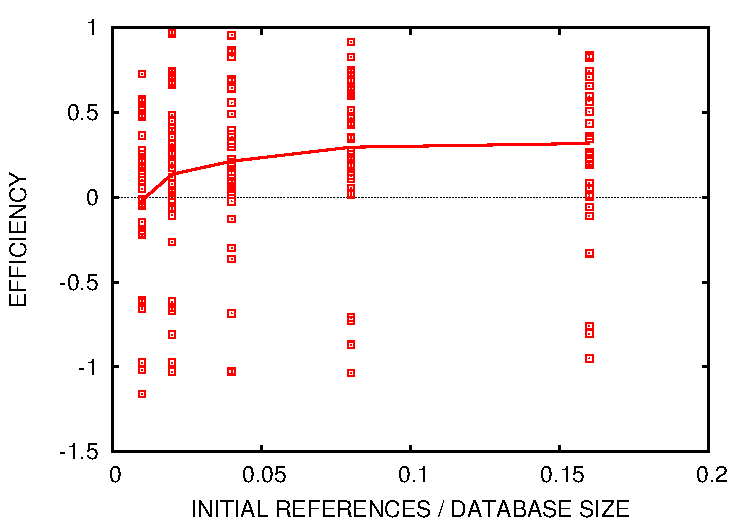
\includegraphics[width=\figwidth]{\figpath/metric_search_efficiency.pdf}}
\caption{Search efficiency as function of the number of groups $k$ in any given level the hierarchical graph representation of the database,
 showing increased efficiency with appropriate selection of $k$.
Efficiency is measured by number of new distance computations relative to the size of the database.
}
\label{fig:search_efficiency}
\end{figure}
%xxxxxxxxxxxxxxxxxxxxxxxxxxxxxxxxxxxxxxxxxxxxxxxxxxxxxxxxxxxxxxxxxxxxxxxxxxx

%===========================================================================
\subsection{Interpolation convergence}
%===========================================================================

Regarding question Q4, \fref{fig:force_interpolation} shows force convergence with the size of the interpolation ball in \eref{eq:force_interpolation}.
The volume of this ball roughly correlates with the number of neighboring clusters used in the RBF interpolation \eqref{eq:force_interpolation} given the fixed cluster database sampling density.
Up to a certain radius, the interpolation converges in accuracy but the improvement eventually decreases with additional, more distant cluster neighbors.
The convergence is strongly dependent on the sampling density of the database, \ie the force error is strongly proportional to the distance to the closest sample (refer to \fref{fig:fvsd} which indicates an upper bound of the convergence with the distance to the closest sample and hence to the density of samples in the database).
In a practical sense, given a static/non-adapting database with a fixed sampling density, \fref{fig:force_interpolation}  show the limits to which the interpolation behavior can be controlled by choosing the interpolation ball radius $R$ and the associated decay parameter $\varsigma$.

%xxxxxxxxxxxxxxxxxxxxxxxxxxxxxxxxxxxxxxxxxxxxxxxxxxxxxxxxxxxxxxxxxxxxxxxxxxxx
\begin{figure}[h]
{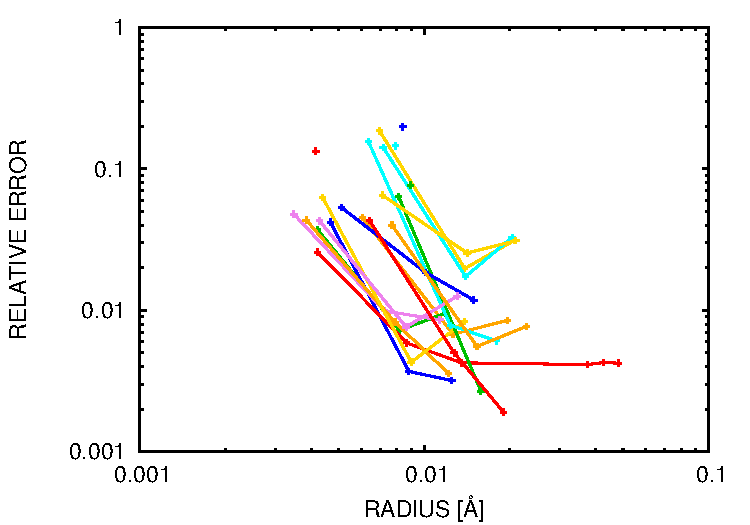
\includegraphics[width=\figwidth]{\figpath/force_error.pdf}}
\caption{Force interpolation accuracy as a function of radius of the interpolation ball $\Bc_Q$ (which correlates with the number of neighboring clusters used in the interpolation). 
Each curve is generated by a different configuration and the error is highly correlated with the distance to the closest cluster in the database.
}
\label{fig:force_interpolation}
\end{figure}
%xxxxxxxxxxxxxxxxxxxxxxxxxxxxxxxxxxxxxxxxxxxxxxxxxxxxxxxxxxxxxxxxxxxxxxxxxxx

%===========================================================================
\subsection{Consistency of dynamics}
%===========================================================================
To test the assembled algorithm and determine the growth rate of the accumulated errors, we created a cluster database from a 100 step (100 fs) \abinitio MD run on a 300 K, $2\!\times\!2\!\times\!2$ unit cell Si system and used this to simulate the dynamics of a $3\!\times\!3\!\times\!3$ system for 200 steps.
In this demonstration no new DFT samples were generated and hence a relatively large interpolation ball was needed (radius 0.02 \AA, in the OGTO metric). 
\fref{fig:dynamics_consistency} shows the temperature and momentum errors relative to a standard \abinitio MD run of the $3\!\times\!3\!\times\!3$  system as a function of time.
Clearly, the temperature error is increasing (linearly) but the momentum error seems to be oscillatory but bounded. 
This apparently unbounded temperature error could be controlled with a thermostat and both errors could be reduced with a denser sampling of cluster space (or an adaptive sampling).


%xxxxxxxxxxxxxxxxxxxxxxxxxxxxxxxxxxxxxxxxxxxxxxxxxxxxxxxxxxxxxxxxxxxxxxxxxxxx
\begin{figure}[h]
{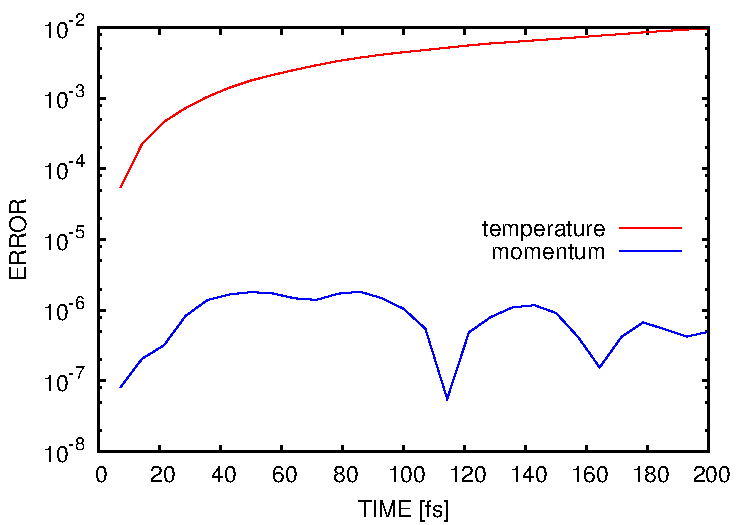
\includegraphics[width=\figwidth]{\figpath/dynamics_error.pdf}}
\caption{ Dynamics consistency: error relative to a full \abinitio dynamics. 
Temperature error normalized by $T=$ 300 K, and momentum error by the average thermal velocity times the mass of the system.
}
\label{fig:dynamics_consistency}
\end{figure}
%xxxxxxxxxxxxxxxxxxxxxxxxxxxxxxxxxxxxxxxxxxxxxxxxxxxxxxxxxxxxxxxxxxxxxxxxxxx

%%%%%%%%%%%%%%%%%%%%%%%%%%%%%%%%%%%%%%%%%%%%%%%%%%%%%%%%%%%%%%%%%%%%%%%%%%%%%%
\section{Discussion} \label{sec:discussion}
%%%%%%%%%%%%%%%%%%%%%%%%%%%%%%%%%%%%%%%%%%%%%%%%%%%%%%%%%%%%%%%%%%%%%%%%%%%%%%

We have set the foundations of a method to simulate molecular dynamics with the accuracy of \abinitio calculations and on the scale of classical molecular dynamics.
The basis of this development is the connection of the local arrangement of atoms to the HF forces on individual atoms. 
Certainly there are materials that violate this condition, \eg those with long range Coulomb interactions and/or extended electronic orbitals, but a large class of important materials are amenable to this treatment and, as mentioned, this connection is the basis for the widely-employed classical molecular dynamics method.
In particular, the proposed method may be effective in simulating metals given the success of the local, empirical embedded atom potential \cite{daw1984embedded}.

In this work we have focussed on the fundamental problem of mapping a local atomic arrangement/configuration to the HF force on central atom.
The basic issue is developing a (I1) translationally, (I2) rotationally, (I3) permutationally invariant method that can be used to drive dynamics or search a database.
We have developed two such methods, one based on the well-known RMS-D metric and the other developed from the OGTO and SOAP similarity measures.
Each has relative advantages. 
RMS-D is cheap to compute including the optimal rotation but finding the optimal permutation remains an issue.
The OGTO metric, on the other hand, is intrinsically permutationally invariant  and has the expected decreasing sensitivity to far away atoms in the local neighborhood at the expense of a more difficult determination of the optimal rotation.
In addition to the two metrics and a version of metric search we provide an accurate means of interpolating forces in neighborhood space.
We have shown: (Q1) the central atom force in a cluster converges to the full system HF force with increasing cluster size, (Q2) the cluster-cluster distances correlate well with the atom forces, (Q3) a metric search is orders of magnitude faster than a brute-force query, and (Q4) with interpolation the error in forces retrieved from the database and the optimal density of the database can be controlled.
These developments allow us to treat the presently infeasible problem of simulating large compositionally and configurationally complex materials with \abinitio accuracy - avoiding the tedious task of constructing a globally applicable empirical potential.
It should be clear that the proposed algorithm reduces to \abinitio molecular dynamics in limit of large neighborhood size and no interpolation.
Our approach, where local interpolations of forces are formed only over the nearest database elements, is distinct from that recently published in \cref{li2015molecular}, where the Gaussian process regression used to form a force field apparently employs the covariance matrix of the entire database. 
Our approach will certainly scale better on supercomputers due to the inherent locality in how the \abinitio data is used and appears to have better accuracy and conservation properties for a given sampling of the \abinitio data. 
%This approach is distinct from the recently published \cref{li2015molecular} in that the local interpolation of forces appears to have better accuracy and conservation properties for a given sampling of the \abinitio data and will certainly scale better on supercomputers due to the inherent locality in how the data is used.
Also we have given explicit details of: (a) how to construct optimal matches between query and database clusters for both RMS-D and OGTO metrics and (b) the metric search and database that enable large-scale computations. 

We leave a number of topics and extensions for future work.
First, although we have some confidence that momentum conservation will be enforced to the degree of error in the HF forces, 
we will need a large-scale  implementation of the algorithm for a complete test of physical momentum and energy conservation with dynamics.
In finite temperature applications we foresee that the conservation properties will be obscured and benefited by thermostat control schemes.
Second, we would like to investigate how to construct a comparison metric appropriate for multi-element materials, which are very challenging to represent in classical formulations of interatomic potentials.
Also, we see that there may be advantages to alternate means of representing cluster space, \eg using the eigen-basis of the cluster graph Laplacian as a basis to embed the cluster manifold in a vector space and drawing upon ideas developed in the context of locality sensitive hashing \cite{leskovec2014mining} to improve the cluster search and force interpolation. % Chap 3
In addition, in following work we will focus on database structure and adaptation. 
Adaptation will be driven by the goal of obtaining optimal density in region of configuration space occupied by the dynamics by pruning configuration samples irrelevant to current state and those in regions that are overly dense that reduce efficiency and adding samples necessary to maintain accuracy.
The basic issue of generating new HF force samples may turn into a significant subsidiary problem in and of itself.
Beyond adapting the database, there are also significant issues in scaling the algorithm to supercomputers, primarily distributing the database across a parallel file-system and managing it in limited memory. 

%%%%%%%%%%%%%%%%%%%%%%%%%%%%%%%%%%%%%%%%%%%%%%%%%%%%%%%%%%%%%%%%%%%%%%%%%%%%%%
\begin{acknowledgement}
%\begin{acknowledgments}
%%%%%%%%%%%%%%%%%%%%%%%%%%%%%%%%%%%%%%%%%%%%%%%%%%%%%%%%%%%%%%%%%%%%%%%%%%%%%%

We appreciate helpful discussions with Aidan Thompson, Kevin Young, Ali Pinar, Jeremy Templeton and Peter Schultz (Sandia), as well as funding from Sandia Laboratories.
Sandia National Laboratories is a multi-program laboratory managed and operated by Sandia Corporation, a wholly owned subsidiary of Lockheed Martin Corporation, for the U.S. Department of Energy's National Nuclear Security Administration under contract DE-AC04-94AL85000.
%Also, we appreciate the scientific software that enabled this project: the DFT data was created with {\sc VASP} (Univ. Vienna), %the MD data with {\sc LAMMPS} (Sandia), the plots with {\sc gnuplot}, and the graph visualizations with {\sc dot} (graphviz).

\end{acknowledgement}
%\end{acknowledgments}

%%%%%%%%%%%%%%%%%%%%%%%%%%%%%%%%%%%%%%%%%%%%%%%%%%%%%%%%%%%%%%%%%%%%%%%%%%%%%%
%\appendix \section{Decomposition of Gaussian overlap inner product} \label{app:soap}
\section*{Appendix: Decomposition of the Gaussian overlap product} \label{app:soap}
%%%%%%%%%%%%%%%%%%%%%%%%%%%%%%%%%%%%%%%%%%%%%%%%%%%%%%%%%%%%%%%%%%%%%%%%%%%%%%%%
A spherical harmonic expansion of the Gaussian-smeared point densities  \eref{eq:sph_harm_expansion}, after dropping the normalization $1/(\sqrt{2\pi}\sigma)^3$ for convenience, can been written:
\begin{equation}
\rho_A(\xb) = 
\sum_{\alpha\in\Nc_A} \exp\left(- \frac{\|\xb-\xb_{\alpha}\|^2}{4 \sigma^2}\right) 
= \sum_{\alpha\in\Nc_A} \left[ \sum_{l=0}^\infty \sum_{m=-l}^l c_\alpha^{lm}(r) Y_{lm} (\rb) \right] , 
\end{equation}
in terms of the spherical harmonic basis $Y_{lm}$ and the coefficients $c_\alpha^{lm}$ containing the corresponding radial series in terms of modified spherical Bessel functions of the 1st kind, $\iota_l$ :
\begin{equation}
c_\alpha^{lm}(r) = 4 \pi 
\exp \left( -\frac{r^2 +r_\alpha^2}{2\sigma^2} \right) 
\iota_l \left(\frac{r r_\alpha}{\sigma^2}\right)  
Y^*_{lm} (\rb_\alpha) 
\end{equation}  
With this expansion we can reformulate the product \eref{eq:ogto_inner_product} and associated norm \eref{eq:ogto_norm}
\begin{equation}
\begin{split}
\langle \rho_A, \rho_B \rangle 
&=
\int \mathrm{d}\xb \rho_A(\xb) \rho_B(\xb)  \\
&= 4 \pi \sum_{\alpha\in\Nc_A} \sum_{\beta\in\Nc_B} 
\exp\left(-\frac{\sigma}{2} (r_\alpha^2 + r_\beta^2) \right)
\sum_{l=0}^{\infty}
\iota_l (\sigma r_\alpha r_\beta) 
\sum_{m=-l}^{l}
Y_{lm} (\rb_\alpha) Y^*_{lm} (\rb_\beta) \\
&= 4 \pi 
\sum_{l=0}^{\infty} \left[
\sum_{\alpha\in\Nc_A} 
\sum_{\beta\in\Nc_B} 
\sum_{m=-l}^{l}
Y_{lm} (\rb_\alpha) 
\exp\left(-\frac{\sigma}{2} r_\alpha^2 \right)
\iota_l (\sigma r_\alpha r_\beta) 
\exp\left(-\frac{\sigma}{2} r_\beta^2 \right)
Y^*_{lm} (\rb_\beta) 
\right] \\
&= \sum_{l=0}^\infty \tr \underbrace{ \left[ \Ys_A \Ws_{AB} \Ys_B^\dagger \right]_l }_{\Js_l}
\end{split}
\end{equation}
with matrices $[\Ys_l]_{\alpha m} = Y_{lm}(\rb_\alpha)$
and $[\Ws_l]_{\alpha\beta} = 4 \pi \exp\left(-\frac{\sigma}{2} (r_\alpha^2) \right)  \iota_l (\sigma r_\alpha r_\beta) \exp\left(-\frac{\sigma}{2} (r_\beta^2) \right)  $.

The rotation of $\neighborhood_B$ relative to $\neighborhood_A$ in the inner product 
\begin{equation}
\begin{aligned}
\left<\rho_A,\Rb \rho_B\right> &= 
\sum_{l=0}^p \sum_{m_A,m_B=-l}^l  D_{l, m_A m_B}(\Rb) \int \mathrm{d}r  
\sum_{\beta_A, \beta_B} c_{\beta_A}^{l, m_A}(r)  c_{\beta_B}^{l, m_B}(r)
\int \mathrm{d}\rb \, Y^*_{l, m_A} (\rb) Y_{l, m_B}(\rb) \\
&= \sum_{l=0}^p \tr \Ds_l(\Rb) \Js_l \ .
\end{aligned}
\end{equation}
can be expressed in terms of \emph{Wigner D} matrices $\Ds_l = \Ds_l(\Rb)$ ($\Ds_l(\Ib)$ is $2l+1$ square identity matrix)
An operational definition of the (unitary) Wigner D matrices is $ \Ys_l(\Rb \rb) = \Ds_l(\Rb) \Ys_l(\rb) $. 
Since  $\Ds_0 = 1 $ is constant and the dimensions of $\Ds_1$ are the same as $\Rb$ albeit being complex valued,
we can find the optimal rotation $\Rb$ that maximizes the similarity $\left<\rho_A,\Rb \rho_B\right>$ via
\begin{equation}
\argmax_\Rb \left<\rho_A,\Rb \rho_B\right>  =
\argmax_\Rb \sum_{l=0}^p \tr \Js_p \Ds_p(\Rb) 
\approx \argmax_\Rb \tr \Js_1 \Ds_1(\Rb)
\end{equation}
First, we apply the mapping $ \Ds_1 = \As^\dagger \Rb \As $ from Eq. 3.63 in \cref{BiedenharnLouck}:
\begin{equation}
\tr \Js_1 \Ds_1
= \tr \Js_1 \As^\dagger \Rb \As  
= \tr \underbrace{ \As \Js_1 \As^\dagger }_{\Ub \Sb \Vb^T} \Rb
\end{equation}
where the transformation matrix $\As: \Ds \rightarrow \Rb$ is constant and unitary.
(We use $\As^*$ to denote the complex conjugate of $\As$ and $\As^\dagger$ to denote the transpose of $\As^*$.)
Hence, an approximate optimal (real-valued) rotation is $\Rb = \Vb \Ub^T$.
Note, given the angle conventions in Biedenharn and Louck's text \cite{BiedenharnLouck}, $\As$ has the components:
\begin{equation}
[ \As ] = 
\begin{bmatrix} 
-1/\sqrt{2} & 0 & 1/\sqrt{2} \\
-\imath/\sqrt{2} & 0 & -\imath/\sqrt{2} \\
0 & 1 & 0
\end{bmatrix}
\end{equation}
Also note given that components of  $\Ys_l$ can be negative implies product formed from truncated SOAP expansion is not metric.

%%%%%%%%%%%%%%%%%%%%%%%%%%%%%%%%%%%%%%%%%%%%%%%%%%%%%%%%%%%%%%%%%%%%%%%%%%%%%%
%% BIBLIOGRAPHY
%%%%%%%%%%%%%%%%%%%%%%%%%%%%%%%%%%%%%%%%%%%%%%%%%%%%%%%%%%%%%%%%%%%%%%%%%%%%%%
\bibliography{Literature/smart_dft_md}
%%%%%%%%%%%%%%%%%%%%%%%%%%%%%%%%%%%%%%%%%%%%%%%%%%%%%%%%%%%%%%%%%%%%%%%%%%%%%%
\end{document}
%%%%%%%%%%%%%%%%%%%%%%%%%%%%%%%%%%%%%%%%%%%%%%%%%%%%%%%%%%%%%%%%%%%%%%%
%% JUNKYARD
%%%%%%%%%%%%%%%%%%%%%%%%%%%%%%%%%%%%%%%%%%%%%%%%%%%%%%%%%%%%%%%%%%%%%%%
